% =================================================================================================
% File:			processi_primari.tex
% Description:	Definisce il capitolo dei processi primari
% Created:		2014-12-11
% Author:		Tesser paolo
% Email:		tesser.paolo@mashup-unipd.it
% =================================================================================================
% Modification History:
% Version		Modifier Date		Change													Author
% 0.0.1 		2014-12-11 			Inizializzazione del file e inizio stesura				Tesser Paolo
% =================================================================================================
% 0.0.2			2014-12-12			continuazione stesura sottosezione fornitura			Tesser Paolo
% =================================================================================================
% 0.0.3			2014-12-12			completamento sottosezione stesura e inizio sviluppo	Tesser Paolo
% =================================================================================================
% 0.0.4			2015-01-08			stesura classificazione requisiti						Tesser Paolo
% =================================================================================================
% 1.0.1			2015-02-25			stesura norme e attività di codifica,progettazione		Faccin Nicola			
% =================================================================================================
% 1.0.2			2015-02-25			inserimento grafici processi primari					Santacatterina Luca			
% =================================================================================================
%


% CONTENUTO DEL CAPITOLO

\section{Processi Primari}
Nella sezione dei Processi Primari sono descritti i processi e le attività che servono alle parti prime durante il ciclo di vita del software. \\
Queste parti sono l'acquirente, il fornitore, lo sviluppatore, l'operatore e il manutentore del prodotto software. \\
Il gruppo \groupName{} si occuperà solo dei Processi di Fornitura e di Sviluppo. Il Processo di Acquisizione spetterà al proponente e al committente del capitolato scelto, mentre il Processo di Manutenzione non potrà essere attuato per vincoli temporali. \\
Nonostante questo l'applicativo \projectName{} e la documentazione fornita con esso dovranno garantire la possibilità futura di procedere con le attività presenti in questo processo a discrezione del proponente.

	\subsection{Processo di fornitura}
		\subsubsection{Attività}

			\paragraph{Accettazione}
				\subparagraph{Discussione e scelta del capitolato}
				Il \roleProjectManager{} ha il compito di organizzare	gli incontri iniziali per permettere ai componenti del gruppo di discutere e esaminare i capitolati selezionati dal committente. \\
				Dalle riunioni emergerà la scelta effettuata dal team. \\
				Le valutazioni che hanno portato a prendere questa decisione verranno documentate in dei verbali.

				\subparagraph{Studio di Fattibilità}
				Agli \emph{Analisti} spetta il compito di redigere lo \docNameVersionSdF{}, basandosi sui verbali citati in precedenza.
Per realizzare il documento dovranno essere presi in considerazione i seguenti punti per ogni capitolato, con maggiore dettaglio per quello preso in carico.
					\begin{itemize}
						\item \textbf{dominio tecnologico e applicativo:} si valutano le conoscenze attuali del team riguardo le tecnologie richieste;
						\item \textbf{interesse strategico:} si valuta quanto interesse abbia il team ad apprendere gli strumenti che serviranno a realizzare il capitolato in questione;
						\item \textbf{rischi possibili:} si analizzano i possibili punti critici in merito anche alle valutazione effettuate nei punti precedenti.
					\end{itemize}
			\paragraph{Preparazione della risposta}
				\subparagraph{Definizione e preparazione della proposta}
				I membri del gruppo \groupName{} dovranno redigere i seguenti documenti: \\
					\begin{itemize}
						\item \docNameVersionSdF
						\item \docNameVersionAdR
						\item \docNameVersionPdP
						\item \docNameVersionPdQ
						\item \docNameVersionNdP
					\end{itemize}
				In allegato a essi si dovrà consegnare una \emph{lettera di presentazione}. \\
				Starà quindi al committente e al proponete valutare l'offerta ricevuta e decidere se accettare o meno la proposta fatta.

			\paragraph{Pianificazione}
				\subparagraph{Scelta del modello di ciclo di vita}
				Il \roleProjectManager{} avrà il compito di scegliere, se non indicato dal proponente, il modello di ciclo di vita adatto per lo sviluppo del prodotto richiesto.
				\subparagraph{Sviluppo e documentazione del Piano di Progetto}
Il \roleProjectManager{} dovrà eseguire una serie di compiti per delineare i lavori che i membri del team dovranno andare ad eseguire, calcolandone i costi e le tempistiche. Il tutto verrà documento nel \docNameVersionPdP{}.

	\subsection{Processo di sviluppo}
		\subsubsection{Attività}
			\paragraph{Analisi dei requisiti}
			Dopo avere redatto lo \docNameSdF{}, agli \emph{Analisti} spetterà il compito di scrivere il documento \docNameVersionAdR{}. \\
			L'obiettivo sarà quello di cercare e produrre dei requisiti a partire dalle informazioni a disposizione del team. \\
			Le risorse che potranno essere utilizzate per questo scopo provengono dal capitolato d'appalto e dagli incontri con il proponente e con il committente. 
			\paragraph{Progettazione}
				\subparagraph{Specifica Tecnica}
				Compito dei \emph{Progettisti} sarà descrivere la progettazione ad alto livello dell'architettura dell'applicazione e dei singoli componenti nella \docNameVersionST. Devono inoltre progettare gli opportuni test di integrazione.\\ \\
					\noindent

					\textbf{Diagrammi UML} \\
					Si utilizzerà il linguaggio UML per definire:
						\begin{itemize}
							\item Diagrammi delle classi;
							\item Diagrammi dei package;
							\item Diagrammi delle attività;
							\item Diagrammi di sequenza;
						\end{itemize}
					Per la stesura, verranno seguite le seguenti convenzioni:
						\begin{itemize}
							\item \textbf{Standard:} standard UML 2.0;
							\item \textbf{Lingua:} la lingua utilizzata è l'inglese.
						\end{itemize}

					\textbf{Design pattern} \\
					La descrizione dei design pattern sarà a carico dei \emph{Progettisti} che sceglieranno quelli più adatti al contesto dell'applicativo per migliorarne l'efficienza. Ogni uno di questi sarà accompagnato da una breve descrizione e da un diagramma che ne esemplificano il funzionamento e la struttura. \\

					\textbf{Tracciamento componenti} \\
					Ogni requisito deve essere tracciato al componente che lo soddisfa. In questo modo sarà possibile misurare il progresso nell’attività di progettazione e garantire che ogni componente soddisfi almeno un requisito.

					\textbf{Test di integrazione} \\
					I \emph{Progettisti} dovranno definire delle classi di verifica, necessarie per verificare che i componenti del sistema funzionino correttamente.

				\subparagraph{Definizione di prodotto}
				Compito dei \emph{Progettisti} sarà descrivere la progettazione a basso livello dell'architettura dell'applicazione nella \docNameVersionDdP, andando ad ampliare quanto descritto nella \docNameVersionST. \\ \\ 

				\textbf{Diagrammi UML} \\
				Si utilizzerà il linguaggio UML per definire:
					\begin{itemize}
						\item Diagrammi delle classi;
						\item Diagrammi delle attività;
						\item Diagrammi di sequenza;
					\end{itemize}

				\textbf{Tracciamento classi} \\
				Ogni requisito deve essere tracciato dalla classe che lo soddisfa. In questo modo sarà possibile misurare il progresso nell’attività di progettazione e garantire che ogni classe soddisfi almeno un requisito.

				\textbf{Test di unità} \\
				I \emph{Progettisti} dovranno definire i test di unità necessari a verificare che i singoli componenti del sistema funzionino nel modo previsto.

			\paragraph{Codifica}
			Le attività di codifica seguiranno svolte dai \emph{Programmatori} dovranno basarsi su quanto descritto nella \docNameVersionDdP{} e seguire le linee guida presenti in questo documento.

		\subsubsection{Procedure}
			\paragraph{Inserimento requisiti nella base di dati}
			Tramite la base di dati creata appositamente è possibile poter inserire nuovi requisiti (figura \ref{fig:procedura_inserimento_requisiti}), l'\roleAnalyst{} deve eseguire le seguenti procedure ordinatamente:

				\begin{enumerate}
			 		\item Accedere alla base usando il link \url{http://gestionale.mashup-unipd.it} ed inserire le credenziali fornite;
			 		\item recarsi nella pagina ``Gestione requisiti";
					\item nella colonna di sinistra selezionare in quale punto dell'albero inserire il nuovo requisito;
					\item cliccare con il tasto destro nel punto identificato e selezionare dal menù a tendina ``Nuovo";
					\item compilare il form con i dati richiesti;
					\item premere salva alla fine del lavoro.
			 	\end{enumerate}

			 	\begin{figure}
					\centering
					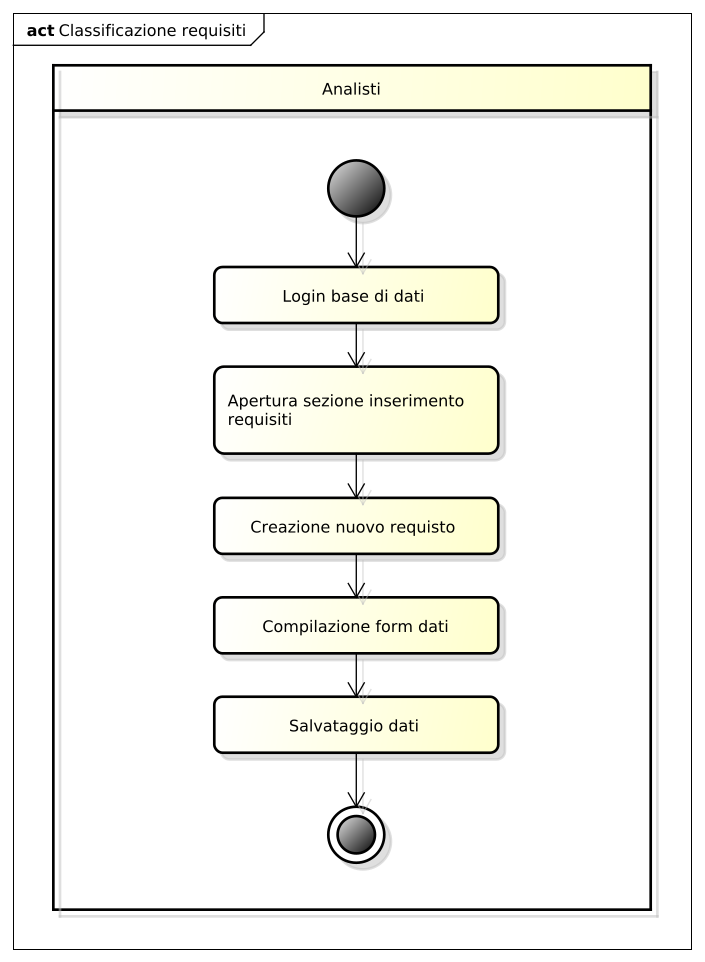
\includegraphics[scale=0.45]{images/classificazione_requisiti.pdf}
					\caption{Diagramma di attività - procedura d'inserimento dei requisiti}
					\label{fig:procedura_inserimento_requisiti}
				\end{figure}

			\paragraph{Inserimento casi d'uso nella base di dati}
			Tramite la base di dati creata appositamente è possibile poter inserire nuovi casi d'uso (figura \ref{fig:procedura_inserimento_uc}), l'\roleAnalyst{} deve eseguire le seguenti procedure ordinatamente:

				\begin{enumerate}
			 		\item accedere alla base usando il link \url{http://gestionale.mashup-unipd.it} ed inserire le credenziali fornite;
			 		\item recarsi nella pagina ``Gestione casi d'uso";
					\item nella colonna di sinistra selezionare in quale punto dell'albero inserire il nuovo caso d'uso;
					\item cliccare con il tasto destro nel punto identificato e selezionare dal menù a tendina ``Nuovo";
					\item compilare il form con i dati richiesti;
					\item premere salva alla fine del lavoro.
			 	\end{enumerate}

			 	\begin{figure}
					\centering
					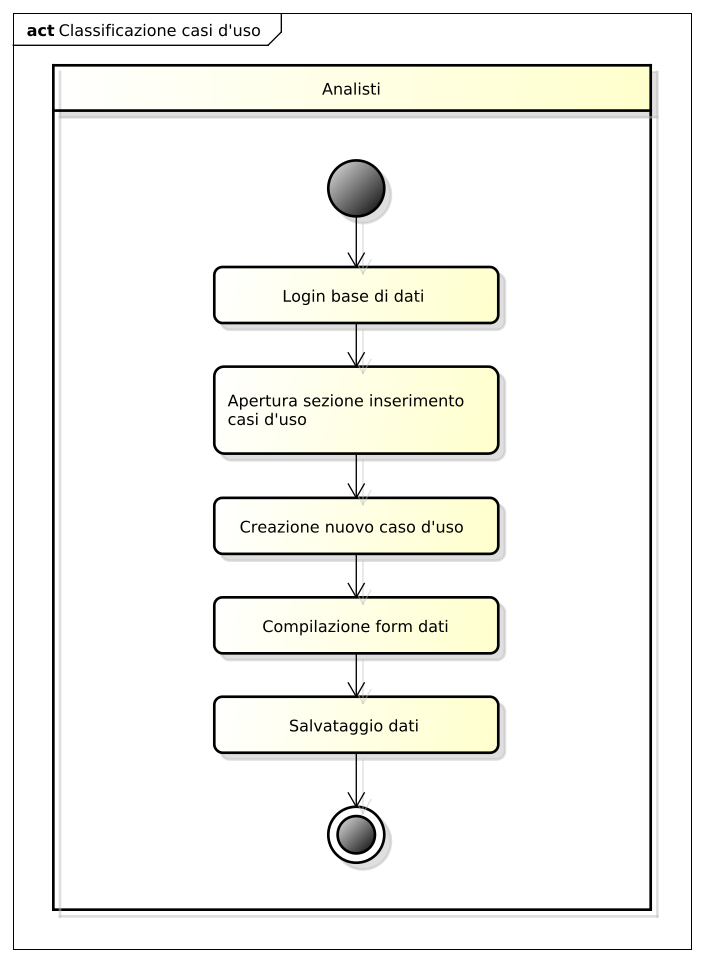
\includegraphics[scale=0.45]{images/classificazione_uc.pdf}
					\caption{Diagramma di attività - procedura d'inserimento dei casi d'uso}
					\label{fig:procedura_inserimento_uc}
				\end{figure}




			\paragraph{Aggiunta template di struttura file in WebStorm} % (fold)
			\label{par:aggiunta_template_di_struttura_file_in_webstorm}
			Di seguito vengono elencati i passi che ogni \roleProgrammer{} dovrà compiere la prima volta che andrà a lavorare sul codice relativo al client dell'applicazione.
				\begin{enumerate}
					\item aprire l'applicativo WebStorm;
					\item aprire il pannello delle preferenze;
					\item selezionare la voce \textbf{File and Code Templates};
					\item premere sul tasto + in verde che dice ``Create Template'';
					\item dare un nome significativo a seconda del tipo che si vuole creare;
					\item copiare uno dei template riportati nell'appendice \ref{sec:configurazione_file_angularjs};
					\item salvare le nuove aggiunte;
					\item ripetere dal passo 4 finché non saranno terminati i template da inserire.
				\end{enumerate}

		 	\begin{figure}
				\centering
				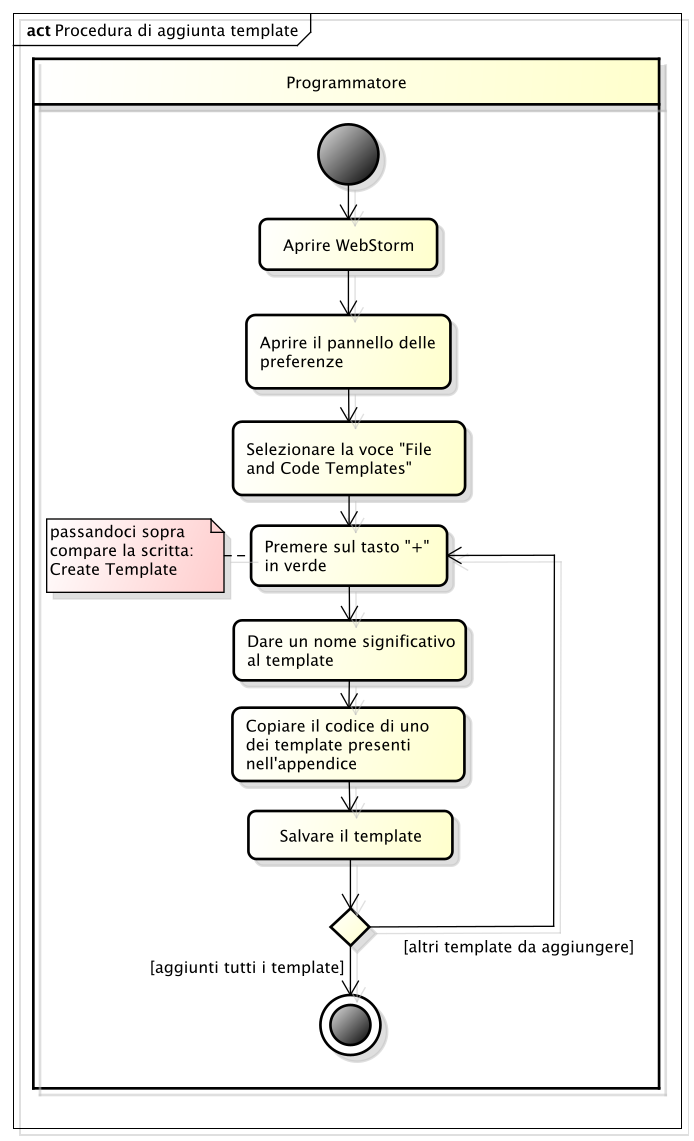
\includegraphics[scale=0.45]{images/proc_aggiunta_template.pdf}
				\caption{Diagramma di attività - procedura di aggiunta template in WebStorm}
				\label{fig:procedura_inserimento_uc}
			\end{figure}
			% paragraph aggiunta_template_di_struttura_file_in_webstorm (end)



		\subsubsection{Norme}
			\paragraph{Classificazione requisiti}
			I requisiti prodotti dovranno essere classificati a seconda del tipo e dell'importanza, seguendo la seguente notazione:
				\begin{center}
					R[Importanza][Tipo][Codice]
				\end{center}
			\noindent
				\begin{itemize}
					\item \textbf{Importanza}: i valori che può assumere sono:
						\begin{itemize}
							\item O: requisito obbligatorio;
							\item D: requisito desiderabile;
							\item F: requisito facoltativo(opzionale).
						\end{itemize}
					\item \textbf{Tipo}: i valori che può assumere sono:
						\begin{itemize}
							\item F: requisito funzionale;
							\item P: requisito prestazionale;
							\item Q: requisito di qualità;
							\item V: requisito di vincolo.
						\end{itemize}
					\item \textbf{Codice}: è il codice gerarchico e univoco del vincolo espresso nella forma X.X.X dove X è un valore numerico.
				\end{itemize}
			\noindent
			Ogni requisito inoltre dovrà contenere le seguente informazioni:
				\begin{itemize}
					\item \textbf{Descrizione}: descrizione del requisito il meno possibile ambigua;
					\item \textbf{Fonte}: la scelta può ricadere tra:
						\begin{itemize}
							\item \textbf{capitolato}: è il requisito che viene trovato dalle specifiche del capitolato di appalto;
							\item \textbf{interno}: è il requisito che viene trovato dagli \emph{Analisti} durante un'analisi più approfondita;
							\item \textbf{caso d'uso}: è il requisito che viene trovato a partire da uno o più casi d'uso. In tal caso andrà specificato il codice del caso d'uso a cui si riferisce;
							\item \textbf{verbale}: è il requisito che viene trovato dagli incontri con il proponente o da incontri interni tra i membri del gruppo.
						\end{itemize}
				\end{itemize}

			\paragraph{Classificazione casi d'uso}
I casi d'uso devono essere divisi in ordine gerarchico secondo il seguente schema: \\
				\begin{center}
					UC[Codice]
				\end{center}
				\begin{itemize}
					\item \textbf{Codice}: è il codice gerarchico e univoco per identificare ogni caso d'uso.
				\end{itemize}
			\noindent Per ogni caso d'uso dovranno essere presenti anche le seguenti informazioni:
				\begin{itemize}
					\item \textbf{titolo}: fornire un titolo riassuntivo dell'operazione che il caso d'uso intende modellare;
					\item \textbf{descrizione}: fornire una breve descrizione del caso d'uso che sia il meno ambigua possibile;
					\item \textbf{attori principali}: elenco degli attori principali coinvolti nel caso d'uso;
					\item \textbf{attori secondari}: elenco degli attori secondari coinvolti nel caso d'uso;
					\item \textbf{scenari principali}: descrizione dei possibili scenari principali;
					\item \textbf{scenari alternativi}: descrizione dei possibili scenari secondari;
					\item \textbf{pre-condizioni}: condizione di partenza sempre vera all'inizio del caso d’uso;
					\item \textbf{flusso degli eventi}: ordine di esecuzione dei casi d'uso figli;
					\item \textbf{inclusioni}: spiegazione di tutte le inclusioni se presenti;
					\item \textbf{estensioni}: spiegazione di tutte le estensioni se presenti;
					\item \textbf{generalizzazioni}: spiegazione di tutte le generalizzazioni, se presenti;;
					\item \textbf{post-condizioni}: condizione finale sempre vera alla fine dell'esecuzione del caso d'uso.
				\end{itemize}
			\noindent
			Alcuni dei campi potranno essere assenti nel caso dovessero risultare inutilizzati.

			\paragraph{Codifica file} % (fold)
			\label{par:codifica}
			Tutti i file che vengono creati, contenenti sia codice sia documentazione, devono essere codificati tramite UTF-8 senza BOM. \\
			Se verrà a verificarsi la necessità di un cambiamento il \roleProjectManager{} ne dovrà approvare le modifiche.
			% paragraph codifica (end)

			\paragraph{Nomi e norme di codifica} % (fold)
			\label{par:nomi_e_norme_di_codifica}
			Il codice dovrà seguire determinate linee guida a seconda del linguaggio.
				\begin{itemize}
					\item \textbf{Python}: Google Python Style Guide \url{https://google-styleguide.googlecode.com/svn/trunk/pyguide.html};
					\item \textbf{Javascript}: Google JavaScript Style Guide \url{http://google-styleguide.googlecode.com/svn/trunk/javascriptguide.xml?showone=Method_and_property_definitions#Method_and_property_definitions};
					\item \textbf{AngularJS}: Google AngularJS Style Guide \url{https://google-styleguide.googlecode.com/svn/trunk/angularjs-google-style.html}.
				\end{itemize}

				\begin{itemize}
					\item ci dovrà essere un header su ciascun file che conterrà le seguente informazioni:
						\begin{itemize}
							\item percorso del file e nome del file;
							\item cognome e nome dell'autore;
							\item data di creazione;
							\item email dell'autore;
							\item dovranno inoltre essere inserite per ogni modifica che verrà effettuata: la successiva versione generata dall'avanzamento, la data, una breve descrizione e l'autore.
						\end{itemize}
					\noindent
					Esempio relativo ai file in Python, ma che dovrà essere simile anche per i file javascript:
					\begin{verbatim}
					# File: nome_del_file
					# Author: Cognome Nome
					# Email: cognome.nome@mashup-unipd.it
					# Date: AAAA-MM-DD
					# Modify:
					# =============================================================
					# Version       Date           Author              Description  
					# =============================================================
					# x.y.z         AAAA-MM-DD     Cognome Nome        Description
					# -------------------------------------------------------------
					\end{verbatim}

					\item i nomi delle variabili dovranno essere in inglese;
					\item i commenti dovranno essere in italiano
				\end{itemize}
			% paragraph nomi_e_norme_di_codifica (end)

			\paragraph{Ricorsione} % (fold)
			\label{par:ricorsione}
			La ricorsione va evitata quando possibile. Per ogni funzione ricorsiva è necessario fornire una prova di terminazione. È inoltre necessario valutare il costo in termini di occupazione della memoria. Nel caso in cui l’utilizzo di memoria risulti troppo elevato, la ricorsione verrà rimossa.
			% paragraph ricorsione (end)

		\subsubsection{Strumenti}

			\paragraph{RequirementsTool}
			\label{par:requirements_tool}
			Il gruppo ha creato un applicativo web che gestisce l'immagazzinamento e il tracciamento dei requisiti e delle fonti attraverso l'inserimento in appositi form. \\
			Il servizio viene offerto nel servizio di hosting del team e ci si può accedere attraverso le API Key di Asana. \\
			L'applicativo è anche in grado di tracciare tutti i task che sono assegnati al membro loggatto e consentire la gestione del tempo di esecuzione di ciascuno di essi. \\
			Lo strumento è scritto in PHP.

			\paragraph{PhpStorm} % (fold)
			\label{par:php_storm}
			L'IDE JetBrains PhpStorm edizione professional, disponibile tramite licenza studentesca, viene utilizzato per scrivere il codice PHP relativo all'applicativo descritto nella sezione \ref{par:requirements_tool}
			\paragraph{PyCharm}
			L'IDE JetBrains PyCharm edizione professional, disponibile tramite licenza studentesca, viene utilizzato per scrivere codice in Python relativo al back-end dell'applicativo.
			\paragraph{WebStorm} % (fold)
			\label{par:webstorm}
			L'IDE JetBrains WebStorm edizione professional, disponibile tramite licenza studentesca, viene utilizzato per il front-end, quindi per il codice in Javascript e HTML
			% paragraph webstorm (end)
			\paragraph{Google App Engine}
			\'E una piattaforma cloud per lo sviluppo e l'hosting di applicazioni, sarà utilizzata principalmente per il back-end.
			% paragraph php_storm (end)

			\paragraph{Yeoman}
			\label{par:yeoman}
			Al fine di creare la struttura di base per l'applicativo web front-end verrà usato il software di scaffolding Yeoman, con il generatore generator-angular. \newline
			Verranno selezionate tra le opzioni proposte di non utilizzare Sass, di includere Bootstrap e tutti i moduli presenti di AngularJS. \newline
			Questo strumento fornisce già dei sistemi incorporati per gestire anche tutta la parte relativa ai test dell'applicazione che verranno spiegati alla sezione \ref{ssub:verifica_strumenti} come Karma, Jasmine e PhantomJS.
